\documentclass[11pt,a4paper]{article}
\usepackage[margin=22mm]{geometry}
\usepackage[T1]{fontenc}
\usepackage[utf8]{inputenc}
\usepackage[british]{babel}
\usepackage{lmodern,microtype,amsmath,amssymb,amsthm,booktabs,tabularx,graphicx,array,longtable}
\usepackage{xcolor,caption,placeins,textcomp,url,seqsplit}
\definecolor{figteal}{HTML}{007F86}
\usepackage[colorlinks=true,linkcolor=figteal,citecolor=figteal,urlcolor=figteal]{hyperref}
\usepackage{xr-hyper}
\def\UrlBreaks{\do\A\do\B\do\C\do\D\do\E\do\F\do\G\do\H\do\I\do\J\do\K\do\L\do\M\do\N\do\O\do\P\do\Q\do\R\do\S\do\T\do\U\do\V\do\W\do\X\do\Y\do\Z\do\a\do\b\do\c\do\d\do\e\do\f\do\g\do\h\do\i\do\j\do\k\do\l\do\m\do\n\do\o\do\p\do\q\do\r\do\s\do\t\do\u\do\v\do\w\do\x\do\y\do\z\do\0\do\1\do\2\do\3\do\4\do\5\do\6\do\7\do\8\do\9\do\/\do\_\do\.\do\-\do\:\do\,\do\(\do\)\do\[\do\]}
\Urlmuskip=0mu plus 1mu
\externaldocument[M-]{build/main}
\hypersetup{pdftitle={Compiling by exact queries over index sets: Supplementary Information},pdfauthor={Alberto Hern\'andez-Espinosa}}
\captionsetup{font=small,labelfont=bf}
\setlength{\parskip}{3pt}
\setlength{\emergencystretch}{3em}
\graphicspath{{generated/}}
\renewcommand{\thesection}{S\arabic{section}}
\renewcommand{\thetable}{S\arabic{table}}
\renewcommand{\thefigure}{S\arabic{figure}}
\newtheorem{proposition}{Proposition}
\renewcommand{\theproposition}{S\arabic{proposition}}
\newcommand{\bits}{\{0,1\}}
\makeatletter
\newcommand{\tableinput}[1]{\@@input #1 }
\makeatother
% Generated by phase2_evidence.Ledger. Do not edit.
\makeatletter
\expandafter\def\csname lv@aZeroAccHi\endcsname{0.0660}
\expandafter\def\csname lv@aZeroAccLo\endcsname{0.0251}
\expandafter\def\csname lv@aZeroAccLog\endcsname{0.0439}
\expandafter\def\csname lv@aZeroAccN\endcsname{100}
\expandafter\def\csname lv@aZeroAccRed\endcsname{4.3}
\expandafter\def\csname lv@aZeroAccTime\endcsname{0.073}
\expandafter\def\csname lv@aZeroAcclosses\endcsname{0}
\expandafter\def\csname lv@aZeroAccties\endcsname{74}
\expandafter\def\csname lv@aZeroAccwins\endcsname{26}
\expandafter\def\csname lv@aZeroClHi\endcsname{0.1194}
\expandafter\def\csname lv@aZeroClLo\endcsname{0.0592}
\expandafter\def\csname lv@aZeroClLog\endcsname{0.0882}
\expandafter\def\csname lv@aZeroClN\endcsname{100}
\expandafter\def\csname lv@aZeroClRed\endcsname{8.4}
\expandafter\def\csname lv@aZeroClTime\endcsname{7.286}
\expandafter\def\csname lv@aZeroCllosses\endcsname{12}
\expandafter\def\csname lv@aZeroClties\endcsname{35}
\expandafter\def\csname lv@aZeroClwins\endcsname{53}
\expandafter\def\csname lv@aZeroPub\endcsname{2.032760}
\expandafter\def\csname lv@bA\endcsname{0.01}
\expandafter\def\csname lv@bB\endcsname{0.1}
\expandafter\def\csname lv@bC\endcsname{1}
\expandafter\def\csname lv@effCeil\endcsname{0.819}
\expandafter\def\csname lv@effPred\endcsname{0.939}
\expandafter\def\csname lv@exAnchor\endcsname{1}
\expandafter\def\csname lv@exFree\endcsname{10}
\expandafter\def\csname lv@exMembers\endcsname{0, 2, 8, 10}
\expandafter\def\csname lv@exRangeHi\endcsname{7}
\expandafter\def\csname lv@exResult\endcsname{0, 2}
\expandafter\def\csname lv@facCat\endcsname{\ensuremath{-}0.0623}
\expandafter\def\csname lv@facCatHi\endcsname{\ensuremath{-}0.0430}
\expandafter\def\csname lv@facCatLo\endcsname{\ensuremath{-}0.0843}
\expandafter\def\csname lv@facInt\endcsname{+0.0075}
\expandafter\def\csname lv@facIntHi\endcsname{+0.0172}
\expandafter\def\csname lv@facIntLo\endcsname{\ensuremath{-}0.0030}
\expandafter\def\csname lv@facPrograms\endcsname{100}
\expandafter\def\csname lv@facTrav\endcsname{+0.0020}
\expandafter\def\csname lv@facTravHi\endcsname{+0.0070}
\expandafter\def\csname lv@facTravLo\endcsname{\ensuremath{-}0.0034}
\expandafter\def\csname lv@feAttempts\endcsname{160,000}
\expandafter\def\csname lv@feBelow\endcsname{4}
\expandafter\def\csname lv@feCaseChecks\endcsname{1,356}
\expandafter\def\csname lv@feCompletions\endcsname{819}
\expandafter\def\csname lv@feDiscrepancies\endcsname{0}
\expandafter\def\csname lv@feExhausted\endcsname{24}
\expandafter\def\csname lv@feFixtures\endcsname{12}
\expandafter\def\csname lv@feMinimum\endcsname{100}
\expandafter\def\csname lv@feRoundTrips\endcsname{564}
\expandafter\def\csname lv@feStreams\endcsname{16}
\expandafter\def\csname lv@hCOne\endcsname{b9697640e202c7cf2563ef3f11423f6cbd52403f91c897b62a6ab1b044672cfa}
\expandafter\def\csname lv@hExpCOne\endcsname{58ee75059dcbdd9f}
\expandafter\def\csname lv@hExpRZero\endcsname{74c87b69e6306359}
\expandafter\def\csname lv@hPOne\endcsname{d14bf39b450aaa5f}
\expandafter\def\csname lv@hRZero\endcsname{d0fcd441886cc5c3}
\expandafter\def\csname lv@ladFourHi\endcsname{+0.0726}
\expandafter\def\csname lv@ladFourLo\endcsname{+0.0442}
\expandafter\def\csname lv@ladFourQ\endcsname{+0.0579}
\expandafter\def\csname lv@ladFourT\endcsname{14.57}
\expandafter\def\csname lv@ladFourlosses\endcsname{0}
\expandafter\def\csname lv@ladFourties\endcsname{107}
\expandafter\def\csname lv@ladFourwins\endcsname{93}
\expandafter\def\csname lv@ladOneHi\endcsname{+0.0091}
\expandafter\def\csname lv@ladOneLo\endcsname{+0.0025}
\expandafter\def\csname lv@ladOneQ\endcsname{+0.0055}
\expandafter\def\csname lv@ladOneT\endcsname{1.17}
\expandafter\def\csname lv@ladOnelosses\endcsname{0}
\expandafter\def\csname lv@ladOneties\endcsname{182}
\expandafter\def\csname lv@ladOnewins\endcsname{18}
\expandafter\def\csname lv@ladThreeHi\endcsname{+0.0000}
\expandafter\def\csname lv@ladThreeLo\endcsname{+0.0000}
\expandafter\def\csname lv@ladThreeQ\endcsname{+0.0000}
\expandafter\def\csname lv@ladThreeT\endcsname{0.83}
\expandafter\def\csname lv@ladThreelosses\endcsname{0}
\expandafter\def\csname lv@ladThreeties\endcsname{200}
\expandafter\def\csname lv@ladThreewins\endcsname{0}
\expandafter\def\csname lv@ladTwoHi\endcsname{+0.0000}
\expandafter\def\csname lv@ladTwoLo\endcsname{\ensuremath{-}0.0028}
\expandafter\def\csname lv@ladTwoQ\endcsname{\ensuremath{-}0.0011}
\expandafter\def\csname lv@ladTwoT\endcsname{0.82}
\expandafter\def\csname lv@ladTwolosses\endcsname{2}
\expandafter\def\csname lv@ladTwoties\endcsname{198}
\expandafter\def\csname lv@ladTwowins\endcsname{0}
\expandafter\def\csname lv@lrnBoundary\endcsname{33}
\expandafter\def\csname lv@lrnEcoPrograms\endcsname{100}
\expandafter\def\csname lv@lrnEcoZero\endcsname{0}
\expandafter\def\csname lv@lrnFixtures\endcsname{30}
\expandafter\def\csname lv@lrnHam\endcsname{\ensuremath{-}0.107}
\expandafter\def\csname lv@lrnHamNeg\endcsname{30}
\expandafter\def\csname lv@lrnQueries\endcsname{1,639}
\expandafter\def\csname lv@lrnRand\endcsname{0.061}
\expandafter\def\csname lv@lrnShuf\endcsname{0.045}
\expandafter\def\csname lv@lvOne\endcsname{98.33}
\expandafter\def\csname lv@lvStd\endcsname{95}
\expandafter\def\csname lv@lvThree\endcsname{97.5}
\expandafter\def\csname lv@lvTwo\endcsname{98.75}
\expandafter\def\csname lv@mBits\endcsname{32}
\expandafter\def\csname lv@mOneSlot\endcsname{1}
\expandafter\def\csname lv@mPublic\endcsname{8}
\expandafter\def\csname lv@mTwoSlot\endcsname{2}
\expandafter\def\csname lv@mVlen\endcsname{8}
\expandafter\def\csname lv@mWords\endcsname{256}
\expandafter\def\csname lv@pOneAccepted\endcsname{18}
\expandafter\def\csname lv@pOneClassical\endcsname{1.901379}
\expandafter\def\csname lv@pOneExtraBoot\endcsname{2.362098}
\expandafter\def\csname lv@pOneExtraCl\endcsname{2.370890}
\expandafter\def\csname lv@pOneExtraFull\endcsname{2.376597}
\expandafter\def\csname lv@pOneExtraN\endcsname{100}
\expandafter\def\csname lv@pOneGain\endcsname{5.63}
\expandafter\def\csname lv@pOneImproved\endcsname{6}
\expandafter\def\csname lv@pOneReps\endcsname{15}
\expandafter\def\csname lv@pOneScore\endcsname{2.008466}
\expandafter\def\csname lv@pOneSlowBoot\endcsname{2.07}
\expandafter\def\csname lv@pOneSlowFull\endcsname{657.5}
\expandafter\def\csname lv@pOneSpeedBoot\endcsname{1.163}
\expandafter\def\csname lv@pOneSpeedFull\endcsname{2.132}
\expandafter\def\csname lv@pOneSpeedFullHi\endcsname{2.138}
\expandafter\def\csname lv@pOneSpeedFullLo\endcsname{2.127}
\expandafter\def\csname lv@pOneTests\endcsname{351}
\expandafter\def\csname lv@pOneWorkerBoot\endcsname{1.134}
\expandafter\def\csname lv@pOneWorkerFull\endcsname{1.947}
\expandafter\def\csname lv@rOneAccHi\endcsname{10.72}
\expandafter\def\csname lv@rOneAccLo\endcsname{6.86}
\expandafter\def\csname lv@rOneAccRed\endcsname{8.76}
\expandafter\def\csname lv@rOneAccTime\endcsname{0.82}
\expandafter\def\csname lv@rOneAccTimeHi\endcsname{0.97}
\expandafter\def\csname lv@rOneAccTimeLo\endcsname{0.68}
\expandafter\def\csname lv@rOneAccTimeThree\endcsname{0.817}
\expandafter\def\csname lv@rOneAcclosses\endcsname{0}
\expandafter\def\csname lv@rOneAccties\endcsname{73}
\expandafter\def\csname lv@rOneAccwins\endcsname{127}
\expandafter\def\csname lv@rOneAzeroHi\endcsname{7.74}
\expandafter\def\csname lv@rOneAzeroLo\endcsname{4.50}
\expandafter\def\csname lv@rOneAzeroRed\endcsname{6.04}
\expandafter\def\csname lv@rOneAzeroTime\endcsname{11.65}
\expandafter\def\csname lv@rOneAzeroTimeHi\endcsname{13.53}
\expandafter\def\csname lv@rOneAzeroTimeLo\endcsname{10.03}
\expandafter\def\csname lv@rOneAzerolosses\endcsname{0}
\expandafter\def\csname lv@rOneAzeroties\endcsname{98}
\expandafter\def\csname lv@rOneAzerowins\endcsname{102}
\expandafter\def\csname lv@rOneBonf\endcsname{99.17}
\expandafter\def\csname lv@rOneClHi\endcsname{12.84}
\expandafter\def\csname lv@rOneClLo\endcsname{8.38}
\expandafter\def\csname lv@rOneClRed\endcsname{10.58}
\expandafter\def\csname lv@rOneClTime\endcsname{76.20}
\expandafter\def\csname lv@rOneClTimeHi\endcsname{92.74}
\expandafter\def\csname lv@rOneClTimeLo\endcsname{62.41}
\expandafter\def\csname lv@rOneCllosses\endcsname{20}
\expandafter\def\csname lv@rOneClties\endcsname{42}
\expandafter\def\csname lv@rOneClwins\endcsname{138}
\expandafter\def\csname lv@rOneDevEffect\endcsname{+0.0663}
\expandafter\def\csname lv@rOneLearnOf\endcsname{30}
\expandafter\def\csname lv@rOneLearnZero\endcsname{0}
\expandafter\def\csname lv@rOnePubAfour\endcsname{2.088945}
\expandafter\def\csname lv@rOnePubAzero\endcsname{2.032760}
\expandafter\def\csname lv@rTwoDfsClL\endcsname{15}
\expandafter\def\csname lv@rTwoDfsClLog\endcsname{0.156}
\expandafter\def\csname lv@rTwoDfsClRed\endcsname{14.4}
\expandafter\def\csname lv@rTwoDfsClT\endcsname{39}
\expandafter\def\csname lv@rTwoDfsClW\endcsname{146}
\expandafter\def\csname lv@rTwoDfsEHi\endcsname{0.9757}
\expandafter\def\csname lv@rTwoDfsEJ\endcsname{0.959}
\expandafter\def\csname lv@rTwoDfsELo\endcsname{0.939}
\expandafter\def\csname lv@rTwoDfsET\endcsname{0.916}
\expandafter\def\csname lv@rTwoDfsEnL\endcsname{14}
\expandafter\def\csname lv@rTwoDfsEnT\endcsname{116}
\expandafter\def\csname lv@rTwoDfsEnW\endcsname{70}
\expandafter\def\csname lv@rTwoDfsHHi\endcsname{0.9997}
\expandafter\def\csname lv@rTwoDfsHJ\endcsname{0.989}
\expandafter\def\csname lv@rTwoDfsHLo\endcsname{0.978}
\expandafter\def\csname lv@rTwoDfsHT\endcsname{0.937}
\expandafter\def\csname lv@rTwoDfsHnL\endcsname{10}
\expandafter\def\csname lv@rTwoDfsHnT\endcsname{161}
\expandafter\def\csname lv@rTwoDfsHnW\endcsname{29}
\expandafter\def\csname lv@rTwoERoute\endcsname{0.80}
\expandafter\def\csname lv@rTwoHi\endcsname{+0.0460}
\expandafter\def\csname lv@rTwoJ\endcsname{0.969}
\expandafter\def\csname lv@rTwoLo\endcsname{+0.0182}
\expandafter\def\csname lv@rTwoLog\endcsname{+0.0312}
\expandafter\def\csname lv@rTwoPubCap\endcsname{2.102747}
\expandafter\def\csname lv@rTwoPubClassical\endcsname{1.901379}
\expandafter\def\csname lv@rTwoPubDfs\endcsname{2.187957}
\expandafter\def\csname lv@rTwoPubDirect\endcsname{2.008466}
\expandafter\def\csname lv@rTwoPubHeap\endcsname{2.088945}
\expandafter\def\csname lv@rTwoQRoute\endcsname{0.98}
\expandafter\def\csname lv@rTwoTime\endcsname{0.978}
\expandafter\def\csname lv@rTwoWTLL\endcsname{22}
\expandafter\def\csname lv@rTwoWTLT\endcsname{123}
\expandafter\def\csname lv@rTwoWTLW\endcsname{55}
\expandafter\def\csname lv@rTwoWorklist\endcsname{4.8}
\expandafter\def\csname lv@rTwoWorklistGate\endcsname{10.0}
\expandafter\def\csname lv@resident\endcsname{8}
\expandafter\def\csname lv@sliceMs\endcsname{2}
\expandafter\def\csname lv@sliceNodes\endcsname{2,048}
\expandafter\def\csname lv@tAccCases\endcsname{277}
\expandafter\def\csname lv@tAccPrograms\endcsname{142}
\expandafter\def\csname lv@tAdapterRows\endcsname{90}
\expandafter\def\csname lv@tAltSeedACostHi\endcsname{0.598}
\expandafter\def\csname lv@tAltSeedBCostHi\endcsname{0.597}
\expandafter\def\csname lv@tAltSeedCCostHi\endcsname{0.598}
\expandafter\def\csname lv@tAuditC\endcsname{143,585}
\expandafter\def\csname lv@tAuditD\endcsname{32,362}
\expandafter\def\csname lv@tAuditM\endcsname{18,219}
\expandafter\def\csname lv@tCFamaliasing\endcsname{0.591}
\expandafter\def\csname lv@tCFamdependency\endcsname{0.642}
\expandafter\def\csname lv@tCFammixed\endcsname{0.536}
\expandafter\def\csname lv@tCFamscalar\endcsname{0.590}
\expandafter\def\csname lv@tCFamvector\endcsname{0.521}
\expandafter\def\csname lv@tCertMedian\endcsname{31,572}
\expandafter\def\csname lv@tCost\endcsname{0.574}
\expandafter\def\csname lv@tCostFour\endcsname{0.5743}
\expandafter\def\csname lv@tCostHi\endcsname{0.598}
\expandafter\def\csname lv@tCostHiFour\endcsname{0.5978}
\expandafter\def\csname lv@tCostLo\endcsname{0.552}
\expandafter\def\csname lv@tCostLoFour\endcsname{0.5518}
\expandafter\def\csname lv@tDevCost\endcsname{0.589}
\expandafter\def\csname lv@tDevGate\endcsname{0.90}
\expandafter\def\csname lv@tDevLogJ\endcsname{\ensuremath{-}0.0173}
\expandafter\def\csname lv@tDevNodesC\endcsname{912}
\expandafter\def\csname lv@tDevNodesR\endcsname{471.5}
\expandafter\def\csname lv@tDevParity\endcsname{300}
\expandafter\def\csname lv@tDevPrograms\endcsname{100}
\expandafter\def\csname lv@tDevWTLL\endcsname{0}
\expandafter\def\csname lv@tDevWTLT\endcsname{256}
\expandafter\def\csname lv@tDevWTLW\endcsname{44}
\expandafter\def\csname lv@tDriftA\endcsname{0.567}
\expandafter\def\csname lv@tDriftB\endcsname{0.538}
\expandafter\def\csname lv@tDriftC\endcsname{0.598}
\expandafter\def\csname lv@tDriftD\endcsname{0.597}
\expandafter\def\csname lv@tExportRows\endcsname{1,248}
\expandafter\def\csname lv@tExportValid\endcsname{1,248}
\expandafter\def\csname lv@tFamilies\endcsname{5}
\expandafter\def\csname lv@tFixedMedC1\endcsname{0.187}
\expandafter\def\csname lv@tFixedMedR0\endcsname{0.362}
\expandafter\def\csname lv@tFixedPctC1\endcsname{1.07}
\expandafter\def\csname lv@tFixedPctR0\endcsname{2.41}
\expandafter\def\csname lv@tGateCost\endcsname{0.80}
\expandafter\def\csname lv@tGateQual\endcsname{1.01}
\expandafter\def\csname lv@tImport\endcsname{0.601}
\expandafter\def\csname lv@tInherited\endcsname{53}
\expandafter\def\csname lv@tJrA\endcsname{0.986}
\expandafter\def\csname lv@tJrB\endcsname{0.991}
\expandafter\def\csname lv@tJrC\endcsname{0.997}
\expandafter\def\csname lv@tKernelMax\endcsname{4.361}
\expandafter\def\csname lv@tKernelMed\endcsname{2.3649}
\expandafter\def\csname lv@tKernelMin\endcsname{0.920}
\expandafter\def\csname lv@tLossNoUnknown\endcsname{10}
\expandafter\def\csname lv@tLossPrograms\endcsname{4}
\expandafter\def\csname lv@tLossRuns\endcsname{17}
\expandafter\def\csname lv@tLossUnknownA\endcsname{0}
\expandafter\def\csname lv@tLossUnknownB\endcsname{6}
\expandafter\def\csname lv@tLossUnknownC\endcsname{7}
\expandafter\def\csname lv@tMCons\endcsname{0.7864}
\expandafter\def\csname lv@tMFamaliasing\endcsname{0.767}
\expandafter\def\csname lv@tMFamdependency\endcsname{0.900}
\expandafter\def\csname lv@tMFammixed\endcsname{0.727}
\expandafter\def\csname lv@tMFamscalar\endcsname{0.831}
\expandafter\def\csname lv@tMFamvector\endcsname{0.721}
\expandafter\def\csname lv@tMGate\endcsname{0.80}
\expandafter\def\csname lv@tMOldAdapter\endcsname{0.7638}
\expandafter\def\csname lv@tMPoint\endcsname{0.6061}
\expandafter\def\csname lv@tMReg\endcsname{0.8268}
\expandafter\def\csname lv@tMReplayOnly\endcsname{0.7650}
\expandafter\def\csname lv@tMWorkloads\endcsname{30}
\expandafter\def\csname lv@tMemMax\endcsname{1.302}
\expandafter\def\csname lv@tMemMed\endcsname{1.051}
\expandafter\def\csname lv@tMemPrograms\endcsname{30}
\expandafter\def\csname lv@tNodes\endcsname{10,000}
\expandafter\def\csname lv@tOrderC1\endcsname{0.577}
\expandafter\def\csname lv@tOrderC1Pairs\endcsname{461}
\expandafter\def\csname lv@tOrderR0\endcsname{0.572}
\expandafter\def\csname lv@tOrderR0Pairs\endcsname{539}
\expandafter\def\csname lv@tPPmax\endcsname{1.076}
\expandafter\def\csname lv@tPPmedian\endcsname{0.554}
\expandafter\def\csname lv@tPPmin\endcsname{0.264}
\expandafter\def\csname lv@tPPq10\endcsname{0.427}
\expandafter\def\csname lv@tPPq90\endcsname{0.878}
\expandafter\def\csname lv@tPPslower\endcsname{7}
\expandafter\def\csname lv@tParityMismatch\endcsname{0}
\expandafter\def\csname lv@tParityPairs\endcsname{1,000}
\expandafter\def\csname lv@tPctHi\endcsname{98.75}
\expandafter\def\csname lv@tPctLo\endcsname{1.25}
\expandafter\def\csname lv@tPerFamily\endcsname{40}
\expandafter\def\csname lv@tProcess\endcsname{0.649}
\expandafter\def\csname lv@tProgBetter\endcsname{25}
\expandafter\def\csname lv@tProgEqual\endcsname{173}
\expandafter\def\csname lv@tProgWorse\endcsname{2}
\expandafter\def\csname lv@tPrograms\endcsname{200}
\expandafter\def\csname lv@tPubC1A\endcsname{2.135}
\expandafter\def\csname lv@tPubC1B\endcsname{2.188}
\expandafter\def\csname lv@tPubC1C\endcsname{2.188}
\expandafter\def\csname lv@tPubR0A\endcsname{2.081}
\expandafter\def\csname lv@tPubR0B\endcsname{2.188}
\expandafter\def\csname lv@tPubR0C\endcsname{2.188}
\expandafter\def\csname lv@tPubSixC1A\endcsname{2.135275}
\expandafter\def\csname lv@tPubSixC1B\endcsname{2.187957}
\expandafter\def\csname lv@tPubSixC1C\endcsname{2.187957}
\expandafter\def\csname lv@tPubSixR0A\endcsname{2.081045}
\expandafter\def\csname lv@tPubSixR0B\endcsname{2.187957}
\expandafter\def\csname lv@tPubSixR0C\endcsname{2.187957}
\expandafter\def\csname lv@tPytest\endcsname{82}
\expandafter\def\csname lv@tQFamaliasing\endcsname{0.991}
\expandafter\def\csname lv@tQFamdependency\endcsname{0.995}
\expandafter\def\csname lv@tQFammixed\endcsname{0.986}
\expandafter\def\csname lv@tQFamscalar\endcsname{0.994}
\expandafter\def\csname lv@tQFamvector\endcsname{0.987}
\expandafter\def\csname lv@tQoneSeed\endcsname{980183}
\expandafter\def\csname lv@tQual\endcsname{0.991}
\expandafter\def\csname lv@tQualFour\endcsname{0.9908}
\expandafter\def\csname lv@tQualHi\endcsname{0.996}
\expandafter\def\csname lv@tQualHiFour\endcsname{0.9964}
\expandafter\def\csname lv@tQualLo\endcsname{0.985}
\expandafter\def\csname lv@tQualLoFour\endcsname{0.9846}
\expandafter\def\csname lv@tRawStdout\endcsname{9,528}
\expandafter\def\csname lv@tReps\endcsname{5}
\expandafter\def\csname lv@tResamples\endcsname{10,000}
\expandafter\def\csname lv@tSeed\endcsname{2026092802}
\expandafter\def\csname lv@tSeed980026C1J\endcsname{1,440}
\expandafter\def\csname lv@tSeed980026C1cycles\endcsname{20}
\expandafter\def\csname lv@tSeed980026C1scratch\endcsname{72}
\expandafter\def\csname lv@tSeed980026R0J\endcsname{1,280}
\expandafter\def\csname lv@tSeed980026R0cycles\endcsname{20}
\expandafter\def\csname lv@tSeed980026R0scratch\endcsname{64}
\expandafter\def\csname lv@tSeed980183C1J\endcsname{924}
\expandafter\def\csname lv@tSeed980183C1cycles\endcsname{22}
\expandafter\def\csname lv@tSeed980183C1scratch\endcsname{42}
\expandafter\def\csname lv@tSeed980183R0J\endcsname{726}
\expandafter\def\csname lv@tSeed980183R0cycles\endcsname{22}
\expandafter\def\csname lv@tSeed980183R0scratch\endcsname{33}
\expandafter\def\csname lv@tSeedHi\endcsname{980199}
\expandafter\def\csname lv@tSeedLo\endcsname{980000}
\expandafter\def\csname lv@tSubstantive\endcsname{975}
\expandafter\def\csname lv@tSummed\endcsname{0.464}
\expandafter\def\csname lv@tTerA\endcsname{0.730}
\expandafter\def\csname lv@tTerAhi\endcsname{493}
\expandafter\def\csname lv@tTerAlo\endcsname{0}
\expandafter\def\csname lv@tTerAms\endcsname{18.0}
\expandafter\def\csname lv@tTerB\endcsname{0.527}
\expandafter\def\csname lv@tTerBhi\endcsname{9,999}
\expandafter\def\csname lv@tTerBlo\endcsname{568}
\expandafter\def\csname lv@tTerBs\endcsname{0.38}
\expandafter\def\csname lv@tTerC\endcsname{0.491}
\expandafter\def\csname lv@tTerChi\endcsname{9,999}
\expandafter\def\csname lv@tTerClo\endcsname{9,999}
\expandafter\def\csname lv@tTerCs\endcsname{1.13}
\expandafter\def\csname lv@tTraces\endcsname{196}
\expandafter\def\csname lv@tWTLAL\endcsname{0}
\expandafter\def\csname lv@tWTLAT\endcsname{850}
\expandafter\def\csname lv@tWTLAW\endcsname{150}
\expandafter\def\csname lv@tWTLBL\endcsname{6}
\expandafter\def\csname lv@tWTLBT\endcsname{871}
\expandafter\def\csname lv@tWTLBW\endcsname{123}
\expandafter\def\csname lv@tWTLCL\endcsname{17}
\expandafter\def\csname lv@tWTLCT\endcsname{947}
\expandafter\def\csname lv@tWTLCW\endcsname{36}
\expandafter\def\csname lv@tWallTimeA\endcsname{0.984}
\expandafter\def\csname lv@tWallTimeB\endcsname{0.854}
\expandafter\def\csname lv@tWallTimeC\endcsname{0.755}
\expandafter\def\csname lv@tZeroNode\endcsname{5}
\expandafter\def\csname lv@tabPPmixedbroadcastCOne\endcsname{9\ensuremath{\times}16}
\expandafter\def\csname lv@tabPPmixedbroadcastCl\endcsname{9\ensuremath{\times}17}
\expandafter\def\csname lv@tabPPmixedbroadcastDi\endcsname{10\ensuremath{\times}24}
\expandafter\def\csname lv@tabPPmixedbroadcastJ\endcsname{144}
\expandafter\def\csname lv@tabPPmixedbroadcastSer\endcsname{11\ensuremath{\times}42}
\expandafter\def\csname lv@tabPPparallelmemoryCOne\endcsname{13\ensuremath{\times}40}
\expandafter\def\csname lv@tabPPparallelmemoryCl\endcsname{14\ensuremath{\times}56}
\expandafter\def\csname lv@tabPPparallelmemoryDi\endcsname{13\ensuremath{\times}40}
\expandafter\def\csname lv@tabPPparallelmemoryJ\endcsname{520}
\expandafter\def\csname lv@tabPPparallelmemorySer\endcsname{21\ensuremath{\times}128}
\expandafter\def\csname lv@tabPPscalardualchainCOne\endcsname{8\ensuremath{\times}3}
\expandafter\def\csname lv@tabPPscalardualchainCl\endcsname{9\ensuremath{\times}5}
\expandafter\def\csname lv@tabPPscalardualchainDi\endcsname{8\ensuremath{\times}3}
\expandafter\def\csname lv@tabPPscalardualchainJ\endcsname{24}
\expandafter\def\csname lv@tabPPscalardualchainSer\endcsname{12\ensuremath{\times}9}
\expandafter\def\csname lv@tabPPscalarpipelineCOne\endcsname{14\ensuremath{\times}6}
\expandafter\def\csname lv@tabPPscalarpipelineCl\endcsname{14\ensuremath{\times}6}
\expandafter\def\csname lv@tabPPscalarpipelineDi\endcsname{14\ensuremath{\times}6}
\expandafter\def\csname lv@tabPPscalarpipelineJ\endcsname{84}
\expandafter\def\csname lv@tabPPscalarpipelineSer\endcsname{18\ensuremath{\times}15}
\expandafter\def\csname lv@tabPPscalarselectsCOne\endcsname{10\ensuremath{\times}5}
\expandafter\def\csname lv@tabPPscalarselectsCl\endcsname{9\ensuremath{\times}6}
\expandafter\def\csname lv@tabPPscalarselectsDi\endcsname{9\ensuremath{\times}6}
\expandafter\def\csname lv@tabPPscalarselectsJ\endcsname{50}
\expandafter\def\csname lv@tabPPscalarselectsSer\endcsname{20\ensuremath{\times}16}
\expandafter\def\csname lv@tabPPvectoraxpyCOne\endcsname{11\ensuremath{\times}16}
\expandafter\def\csname lv@tabPPvectoraxpyCl\endcsname{10\ensuremath{\times}32}
\expandafter\def\csname lv@tabPPvectoraxpyDi\endcsname{10\ensuremath{\times}24}
\expandafter\def\csname lv@tabPPvectoraxpyJ\endcsname{176}
\expandafter\def\csname lv@tabPPvectoraxpySer\endcsname{14\ensuremath{\times}73}
\expandafter\def\csname lv@tabPPvectorbitmixCOne\endcsname{13\ensuremath{\times}24}
\expandafter\def\csname lv@tabPPvectorbitmixCl\endcsname{10\ensuremath{\times}40}
\expandafter\def\csname lv@tabPPvectorbitmixDi\endcsname{10\ensuremath{\times}40}
\expandafter\def\csname lv@tabPPvectorbitmixJ\endcsname{312}
\expandafter\def\csname lv@tabPPvectorbitmixSer\endcsname{16\ensuremath{\times}89}
\expandafter\def\csname lv@tabPPvectorreductionCOne\endcsname{12\ensuremath{\times}32}
\expandafter\def\csname lv@tabPPvectorreductionCl\endcsname{12\ensuremath{\times}40}
\expandafter\def\csname lv@tabPPvectorreductionDi\endcsname{12\ensuremath{\times}40}
\expandafter\def\csname lv@tabPPvectorreductionJ\endcsname{384}
\expandafter\def\csname lv@tabPPvectorreductionSer\endcsname{19\ensuremath{\times}137}
\expandafter\def\csname lv@tabPubSerial\endcsname{1.000000}
\expandafter\def\csname lv@weC1C\endcsname{9}
\expandafter\def\csname lv@weC1J\endcsname{144}
\expandafter\def\csname lv@weC1S\endcsname{16}
\expandafter\def\csname lv@weCapCcap\endcsname{17}
\expandafter\def\csname lv@weCapJ\endcsname{240}
\expandafter\def\csname lv@weCapLC\endcsname{9}
\expandafter\def\csname lv@weCapLS\endcsname{8}
\expandafter\def\csname lv@weCapScap\endcsname{26}
\expandafter\def\csname lv@weCatalogue\endcsname{11}
\expandafter\def\csname lv@weChildCerts\endcsname{3}
\expandafter\def\csname lv@weChildOp\endcsname{0}
\expandafter\def\csname lv@weChildVal\endcsname{2}
\expandafter\def\csname lv@weClassicalC\endcsname{9}
\expandafter\def\csname lv@weClassicalJ\endcsname{153}
\expandafter\def\csname lv@weClassicalS\endcsname{17}
\expandafter\def\csname lv@weCombDeclared\endcsname{7,873,200}
\expandafter\def\csname lv@weCombRoot\endcsname{972,000}
\expandafter\def\csname lv@weDirectphase1C\endcsname{10}
\expandafter\def\csname lv@weDirectphase1J\endcsname{240}
\expandafter\def\csname lv@weDirectphase1S\endcsname{24}
\expandafter\def\csname lv@weEdges\endcsname{7}
\expandafter\def\csname lv@weEpochs\endcsname{4}
\expandafter\def\csname lv@weHorizon\endcsname{17}
\expandafter\def\csname lv@weImprovements\endcsname{3}
\expandafter\def\csname lv@weLooksC\endcsname{3}
\expandafter\def\csname lv@weLooksR\endcsname{14}
\expandafter\def\csname lv@weNodes\endcsname{5,476}
\expandafter\def\csname lv@weOps\endcsname{8}
\expandafter\def\csname lv@wePubC1Fullcycles\endcsname{9}
\expandafter\def\csname lv@wePubC1Fullscratch\endcsname{16}
\expandafter\def\csname lv@wePubC1Shortcycles\endcsname{10}
\expandafter\def\csname lv@wePubC1Shortscratch\endcsname{16}
\expandafter\def\csname lv@wePubR0Fullcycles\endcsname{9}
\expandafter\def\csname lv@wePubR0Fullscratch\endcsname{16}
\expandafter\def\csname lv@wePubR0Shortcycles\endcsname{10}
\expandafter\def\csname lv@wePubR0Shortscratch\endcsname{17}
\expandafter\def\csname lv@weQAchosen\endcsname{16}
\expandafter\def\csname lv@weQAhi\endcsname{16}
\expandafter\def\csname lv@weQTchosen\endcsname{1}
\expandafter\def\csname lv@weQThi\endcsname{7}
\expandafter\def\csname lv@weQTlo\endcsname{0}
\expandafter\def\csname lv@weQTop\endcsname{2}
\expandafter\def\csname lv@weQTsurv\endcsname{3}
\expandafter\def\csname lv@weQone980026C\endcsname{23}
\expandafter\def\csname lv@weQone980026J\endcsname{1,840}
\expandafter\def\csname lv@weQone980026S\endcsname{80}
\expandafter\def\csname lv@weQone980183C\endcsname{22}
\expandafter\def\csname lv@weQone980183J\endcsname{968}
\expandafter\def\csname lv@weQone980183S\endcsname{44}
\expandafter\def\csname lv@weQueries\endcsname{15}
\expandafter\def\csname lv@weRootCerts\endcsname{5}
\expandafter\def\csname lv@weScaleFinalJ\endcsname{384}
\expandafter\def\csname lv@weScaleFirstJ\endcsname{480}
\expandafter\def\csname lv@weScaleNodes\endcsname{9,999}
\expandafter\def\csname lv@weScaleOps\endcsname{19}
\expandafter\def\csname lv@weSerialC\endcsname{11}
\expandafter\def\csname lv@weSerialJ\endcsname{462}
\expandafter\def\csname lv@weSerialS\endcsname{42}
\expandafter\def\csname lv@weStarterC\endcsname{11}
\expandafter\def\csname lv@weStarterJ\endcsname{462}
\expandafter\def\csname lv@weStarterS\endcsname{42}
\expandafter\def\csname lv@weStarterScore\endcsname{1.000000}
\expandafter\def\csname lv@weStepAC\endcsname{10}
\expandafter\def\csname lv@weStepAS\endcsname{17}
\expandafter\def\csname lv@weStepBC\endcsname{9}
\expandafter\def\csname lv@weStepBS\endcsname{17}
\expandafter\def\csname lv@weStepCC\endcsname{9}
\expandafter\def\csname lv@weStepCS\endcsname{16}
\expandafter\def\csname lv@weSubC\endcsname{4,440}
\expandafter\def\csname lv@weSubCerts\endcsname{1,655}
\expandafter\def\csname lv@weSubChildren\endcsname{3,001}
\expandafter\def\csname lv@weSubR\endcsname{27,874}
\expandafter\def\csname lv@weSubRatio\endcsname{0.16}
\expandafter\def\csname lv@weTimeC1\endcsname{100.4}
\expandafter\def\csname lv@weTimeC1Full\endcsname{233.5}
\expandafter\def\csname lv@weTimeC1Short\endcsname{10.4}
\expandafter\def\csname lv@weTimeClassical\endcsname{0.154}
\expandafter\def\csname lv@weTimeDirect\endcsname{441.680}
\expandafter\def\csname lv@weTimeR0\endcsname{100.5}
\expandafter\def\csname lv@weTimeR0Full\endcsname{239.7}
\expandafter\def\csname lv@weTimeR0Short\endcsname{10.4}
\expandafter\def\csname lv@weTimeSerial\endcsname{0.015}
\newcommand{\V}[1]{\ifcsname lv@#1\endcsname\csname lv@#1\endcsname\else\PackageError{ledger}{Undefined ledger value #1}{}\fi}
\makeatother

\newcommand{\ci}[2]{[#1,\,#2]}
\makeatletter\renewcommand*\l@section{\@dottedtocline{1}{0em}{2.6em}}\makeatother

\title{Compiling by exact queries over index sets\\[4pt]\large Supplementary Information}
\author{Alberto Hern\'andez-Espinosa}
\date{September 2026}

\begin{document}
\maketitle
\tableofcontents

\section{Cube algebra and queries}\label{sec:algebra}

This section completes the algebra of Section~\ref{M-sec:index} of the main text.
Cubes, covers and their notation are as defined there.

\begin{proposition}[Exact disjoint difference]
Subtracting a cube $d$ from a cube $c$ of the same width yields an exact disjoint
cover of $c\setminus d$ with at most $n$ cubes when they intersect, and $c$
itself when they do not.
\end{proposition}
\begin{proof}
Consider, in ascending order, the coordinates that are free in $c$ but fixed in
$d$. At each, emit the part of the current cube that takes the value opposite to
$d$, and continue with the part that agrees. Emitted parts first disagree with $d$
at different coordinates and are therefore disjoint. Every member of $c\setminus
d$ has exactly one first such disagreement, and the final agreeing part lies
inside $d$ and is discarded. There are at most $n$ split coordinates; with none,
$c\subseteq d$ and the result is empty.
\end{proof}

Restricting a coordinate is intersection with that coordinate's literal cube. An
integer interval of a field is decomposed into aligned binary blocks, each a cube
over the field with all other coordinates free. Covers may overlap, so their
sizes cannot in general be added to obtain the size of a union.

\begin{proposition}[Query soundness and conditional completeness]
If every leaf denotes its predicate exactly, every cube returned by the
depth-first solver is contained in the denotation of the query. If the finite
search is exhausted without a resource limit, the absence of an accepting branch
proves the query unsatisfiable in its declared universe.
\end{proposition}
\begin{proof}
The current cube starts as the universe. A leaf intersection keeps exactly the
indices that satisfy the leaf; AND requires every child and OR enumerates the
union of its children. By induction over the pending expression each branch
preserves these set identities, so a completed branch contains only satisfying
indices, and exhausting all branches accounts for the whole expression.
\end{proof}

The first depth-first witness is not guaranteed to be the globally smallest
index; the first answer of the main text uses complete covers and their smallest
anchors, which Proposition~\ref{M-prop:algebra} of the main text makes exact. A
timeout or a count limit is reported as unknown, never as unsatisfiable, and
unsatisfiability refers only to the declared domains and the fixed context.

\section{A representation limit: parity}\label{sec:parity}

\begin{proposition}[Parity needs an exponential flat cube cover]
For $n\geq1$, every exact union of cubes equal to the set of odd-parity indices
consists of $2^{n-1}$ singleton cubes.
\end{proposition}
\begin{proof}
A cube with a free coordinate contains two indices that differ only there, and
they have opposite parity, so it is not a subset of the odd-parity set. In an
exact union every cube must be such a subset, since a union cannot cancel an
unwanted member. Every cube is therefore a singleton, and there are $2^{n-1}$
odd-parity indices.
\end{proof}

\begin{figure}[htbp]\centering
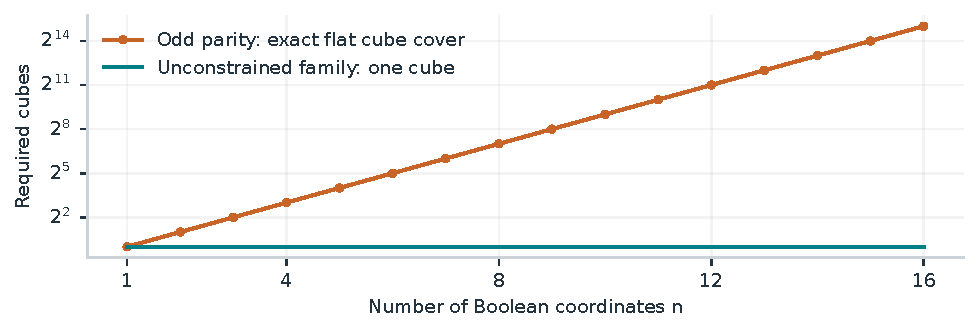
\includegraphics[width=.8\linewidth]{representation_limits.pdf}
\caption{Analytic illustration, not a compiler measurement: an unconstrained
family is one cube, while an exact flat cover of odd parity needs exponentially
many. The bound is specific to flat unions of cubes; it does not establish the
same growth for factored expressions or decision diagrams.}\label{fig:parity}
\end{figure}

A cube with $k$ free coordinates describes $2^k$ indices with two integers, but
that is a saving of representation, not $2^k$ answers computed at constant cost;
expanding the members takes at least their number, and for unbounded widths the
integer operations themselves scale with the number of machine words. Compression
must therefore be stated for a named representation and a named family of
predicates, and the parity example is why.

\begin{figure}[htbp]\centering
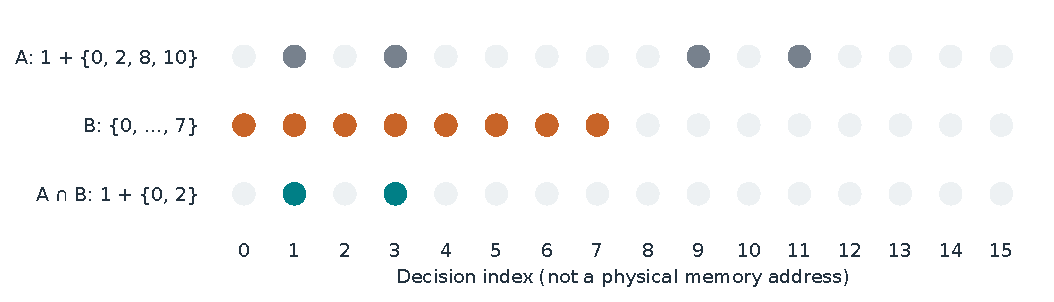
\includegraphics[width=.8\linewidth]{schema_example.pdf}
\caption{A four-coordinate example of the cube algebra: anchor \V{exAnchor} with free mask \V{exFree}
denotes \V{exAnchor} plus each of \{\V{exMembers}\}; intersecting it with the indices up to \V{exRangeHi} leaves
\V{exAnchor} plus each of \{\V{exResult}\}, which is again a cube. The dots expand the sets for reading.}
\label{fig:schema}
\end{figure}

\section{Round one: the ladder}\label{sec:ladder}

Round one fixed five solvers before measuring anything, each adding one
mechanism to the one below, so that adjacent arms form an ablation. A0 is the
structural-encoding search of Phase~2; A1 removes its query cap; A2 replaces the
target rectangles by one strict-product domain per window~\cite{castaneda2019}; A3
adds four certified propagation rules~\cite{ohrimenko2009}; A4 adds a multiscale
catalogue of related windows~\cite{shaw1998} and a discrepancy-ordered
traversal~\cite{harvey1995}. The arm with the largest mean paired
$\log(J_{\mathrm{A0}}/J_{\mathrm{arm}})$ at \V{bB}\,s on \V{tDevPrograms} development
programs was selected (A4, development effect \V{rOneDevEffect}), frozen, and then
measured on \V{tPrograms} fresh programs.

\begin{table}[htbp]\centering\small
\begin{tabular}{lrrrr}\toprule
Step (\V{tPrograms} fresh, \V{bB}\,s) & Mean log $J$ ratio & \V{lvStd}\% interval & W / T / L & Time ratio\\\midrule
A1 over A0 & \V{ladOneQ} & \ci{\V{ladOneLo}}{\V{ladOneHi}} & \V{ladOnewins} / \V{ladOneties} / \V{ladOnelosses} & \V{ladOneT}\\
A2 over A1 & \V{ladTwoQ} & \ci{\V{ladTwoLo}}{\V{ladTwoHi}} & \V{ladTwowins} / \V{ladTwoties} / \V{ladTwolosses} & \V{ladTwoT}\\
A3 over A2 & \V{ladThreeQ} & \ci{\V{ladThreeLo}}{\V{ladThreeHi}} & \V{ladThreewins} / \V{ladThreeties} / \V{ladThreelosses} & \V{ladThreeT}\\
A4 over A3 & \V{ladFourQ} & \ci{\V{ladFourLo}}{\V{ladFourHi}} & \V{ladFourwins} / \V{ladFourties} / \V{ladFourlosses} & \V{ladFourT}\\
\bottomrule\end{tabular}
\caption{Each step against the one below it. Positive log ratios mean the step
lowered $J$. Time ratios are geometric means of per-program median compile times,
step over previous.}\label{tab:ladder}
\end{table}

A2 did not raise quality because the gaps in the target rectangles, though real
in geometry, rarely held improvements on this generator; it did replace a
heuristic refusal by a proof of emptiness and made each query cheaper. A3 changed
no answer at all, which is what a sound propagator should do when every query
already finishes: it can change when an answer is found but not which. The whole
gain of the round is the last step, which bundles two mechanisms; round two took
them apart. The primary comparisons of the round, with Bonferroni-adjusted \V{lvOne}\%
intervals, are in Table~\ref{M-tab:pairs} of the main text; A4 had the best average
output quality among A0, the accepted Phase~1 optimiser and the classical compiler
at \V{bB}\,s on that population, but lost to classical on \V{rOneCllosses} programs and
took \V{rOneClTime} times its compile time.

\begin{figure}[htbp]\centering
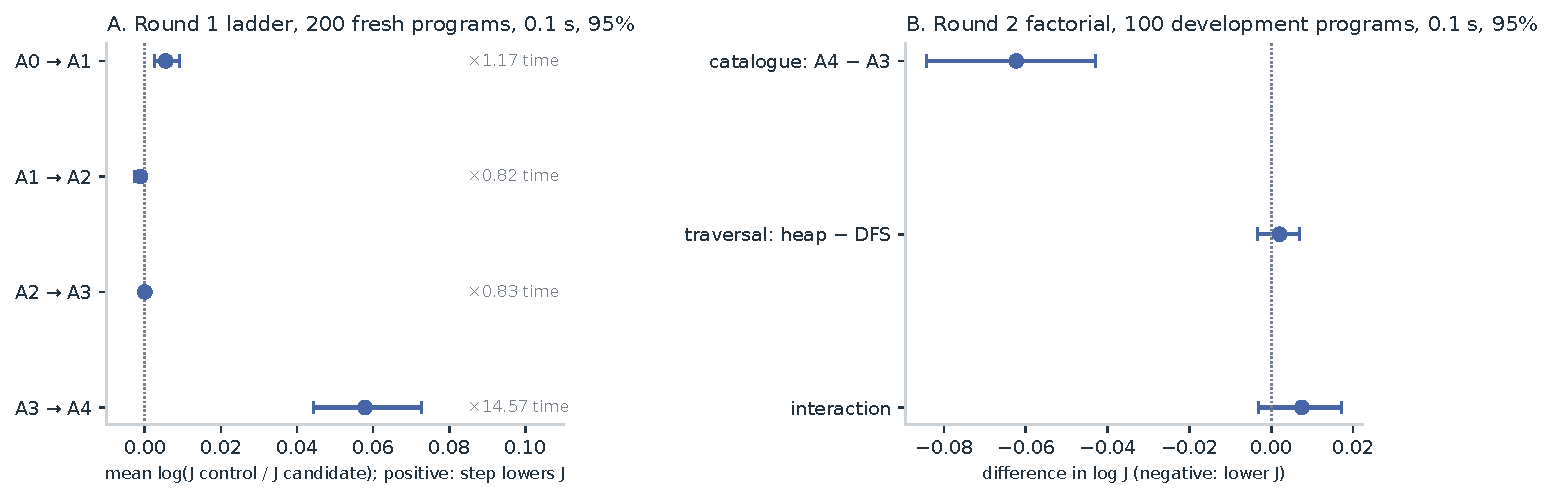
\includegraphics[width=\linewidth]{supp_ladder_factorial.pdf}
\caption{(A)~The round-one ladder, each step against the one below it, with its
compile-time ratio. (B)~The round-two factorial on development programs: the
catalogue lowers $\log J$ and its interval excludes zero; the traversal and the
interaction intervals span zero. The generator checks both statements before
rendering.}\label{fig:ladder}
\end{figure}

\section{Round two: repair, reversal and the factorial}\label{sec:round2}

Review of round one found that interrupted candidate validations were not counted
when no learner was attached; decisions were unaffected, but the report said
zero where the truth was one or more. The repair lives in a versioned successor
that makes the same decisions node for node on a deterministic clock.

\paragraph{A reversal.} On \V{tPrograms} fresh programs the repaired A4 beat the
earlier \texttt{cap512\_wider} optimiser (the Phase~2 controller with a larger query
cap and wider windows): mean log $J$ ratio \V{rTwoLog}, \V{lvStd}\% interval
\ci{\V{rTwoLo}}{\V{rTwoHi}}, J ratio \V{rTwoJ}, with \V{rTwoWTLW} programs better,
\V{rTwoWTLT} equal and \V{rTwoWTLL} worse, at \V{rTwoTime} times its compile time. On
the public suite the order reversed: \V{rTwoPubCap} for \texttt{cap512\_wider}
against \V{rTwoPubHeap} for A4. Both results are exact; one concerns a generator
population and the other eight fixed programs.

\paragraph{The factorial.} Crossing catalogue (A3's small windows or A4's
multiscale catalogue) with traversal (depth-first or discrepancy heap) on
\V{facPrograms} development programs gave a catalogue effect of \V{facCat} in log
$J$ (\ci{\V{facCatLo}}{\V{facCatHi}}), a traversal effect of \V{facTrav}
(\ci{\V{facTravLo}}{\V{facTravHi}}) and an interaction of \V{facInt}
(\ci{\V{facIntLo}}{\V{facIntHi}}). The catalogue explains the gain; the traversal
is not shown to contribute, although its interval does not exclude a small effect.

\paragraph{The selected candidate.} The development rule selected
\texttt{cell\_a4cat\_dfs}, A4's catalogue with depth-first search. On the fresh
cohort its $J$ ratio against heap A4 was \V{rTwoDfsHJ} (\V{lvTwo}\% interval
\ci{\V{rTwoDfsHLo}}{\V{rTwoDfsHHi}}) and against \texttt{cap512\_wider} \V{rTwoDfsEJ}.
Both registered routes to a ``better'' claim required either an upper $J$ bound of at
most \V{rTwoQRoute} or an upper compile-time bound of at most \V{rTwoERoute} at no
loss of quality; neither was met, and the verdict was TARGET\_NOT\_REACHED. The
candidate became R0 after the assurance round.

\paragraph{Learning.} A depth-three schema tree over the code's own
bits~\cite{breiman1984}, used as a guide for exact search in the spirit
of~\cite{gasse2019}, was compared with Hamming order, random order and a tree fitted
on shuffled labels. It beat random order (\V{lrnRand}) and shuffled labels
(\V{lrnShuf}, below the registered minimum), but lost to Hamming order on all
\V{lrnHamNeg} of \V{lrnFixtures} fixtures (\V{lrnHam}). Inside real compilations, not
one of \V{lrnEcoPrograms} programs had a query that reached the required number of
validated observations, and only \V{lrnBoundary} of \V{lrnQueries} learner queries
reached the decision point: ECONOMICALLY\_UNAVAILABLE. The review showed why: under
sound bounds only strict improvements reach the observation hook, and the first
accepted improvement ends the epoch, so at most one observation can exist when the
learner is first prepared. Round one's learning hypothesis had failed by design,
since none of its \V{rOneLearnOf} fixtures contained a test solution better than the
training minimum. The per-query learner is retired for this architecture; other
learning architectures are not ruled out.

\paragraph{Engineering.} Propagation became about three-quarters of profiled
compile time with the multiscale catalogue. A worklist fixed point saved
\V{rTwoWorklist}\% of compile time against a gate of \V{rTwoWorklistGate}\%, and the
parent was kept. The following assurance round proposed a filter on the capacity
rule whose predicted fixed-work ratio was \V{effPred} (with a ceiling of
\V{effCeil} had the scan vanished entirely), against a gate of \V{tGateCost}:
NO\_JUSTIFIED\_OPTIMIZATION.

\section{The third round in detail}\label{sec:third}

\paragraph{The mechanism decision.} Before any integration, a cost model predicted
C1's fixed-work ratio from replays of captured propagation work. The registered
formula gave a conservative \V{tMReg} against a gate of \V{tMGate} and stopped the
round. Review found that the subtracted term covered a narrower scope than the
replayed work, so that overlapping work was charged twice, and that the adapter
cost had been estimated with a loop that did not perform the real operations. The
correction, admitted by the lead reviewer as post-hoc development accounting,
re-measured the adapter in \V{tAdapterRows} fresh processes and gave a conservative
\V{tMCons} (point \V{tMPoint}); the same scope correction with the old adapter gave
\V{tMOldAdapter}, and a replay-only sensitivity \V{tMReplayOnly}. By family the
corrected conservative forecasts were \V{tMFamscalar} (scalar), \V{tMFamvector}
(vector), \V{tMFammixed} (mixed), \V{tMFamdependency} (dependency) and
\V{tMFamaliasing} (aliasing). These are forecasts on \V{tMWorkloads} development
programs, not measurements or confidence bounds. The replay itself reproduced R0's
outputs and certificate streams identically, with a median kernel speed-up of
\V{tKernelMed} (range \V{tKernelMin} to \V{tKernelMax}); an earlier summary had
reported the upper median of the \V{tMWorkloads} values instead.

\paragraph{Development.} On \V{tDevPrograms} development programs, \V{tDevParity}
fixed-work pairs were identical, the fixed-work cost ratio was \V{tDevCost} against a
gate of \V{tDevGate}, and the mean log $J$ ratio at \V{bB}\,s was \V{tDevLogJ} with
\V{tDevWTLW} programs better, \V{tDevWTLT} equal and \V{tDevWTLL} worse. At equal wall
time C1 completed more search (median \V{tDevNodesC} nodes against \V{tDevNodesR}).

\paragraph{Confirmation by family.} The cost ratio was \V{tCFamscalar} (scalar),
\V{tCFamvector} (vector), \V{tCFammixed} (mixed), \V{tCFamdependency} (dependency) and
\V{tCFamaliasing} (aliasing); the quality ratio was \V{tQFamscalar}, \V{tQFamvector},
\V{tQFammixed}, \V{tQFamdependency} and \V{tQFamaliasing} in the same order. Median
fixed-work compile calls were \V{tFixedMedC1}\,s for C1 and \V{tFixedMedR0}\,s for R0,
with ninety-fifth percentiles of \V{tFixedPctC1}\,s and \V{tFixedPctR0}\,s. By search-size
third, R0's median compile call was \V{tTerAms}\,ms on the smallest third,
\V{tTerBs}\,s on the middle third and \V{tTerCs}\,s on the largest; the summed-seconds
ratio was \V{tSummed}. Other allowances: $J$ ratio \V{tJrA} at \V{bA}\,s (\V{tWTLAW}
better, \V{tWTLAT} equal, \V{tWTLAL} worse) and \V{tJrC} at \V{bC}\,s (\V{tWTLCW}, \V{tWTLCT},
\V{tWTLCL}).

\section{Phase 1: the original direct compiler}\label{sec:phase1}

The first version was accepted with limitations after an independent lead review
of its implementation and evidence. Its verifier passed \V{pOneTests} recorded tests
and its standalone export passed the acceptance corpus. On the public suite its
score was \V{pOneScore} against \V{pOneClassical} for classical, a composite-score
advantage of \V{pOneGain}\% that already arises in the first answer; the bounded
optimiser added nothing on the public programs and improved \V{pOneImproved} of
\V{pOneExtraN} generated programs. The score gain is not an execution speed-up and
cannot be attributed to the representation alone, because the two compilers also
use different heuristics.

Implementation refinements then reduced its full compile time by a factor of
\V{pOneSpeedFull} relative to its previous version (paired \V{lvStd}\% interval
\ci{\V{pOneSpeedFullLo}}{\V{pOneSpeedFullHi}}, \V{pOneReps} repetitions per program), and
bootstrap time by \V{pOneSpeedBoot}; an earlier run of the same code gave
\V{pOneWorkerFull} and \V{pOneWorkerBoot}, so within-run intervals understate
between-run variation. Compilation remained much slower than classical: the
geometric means of per-program median candidate/classical ratios were
\V{pOneSlowBoot} for bootstrap and \V{pOneSlowFull} for full compilation.

\begin{figure}[htbp]\centering
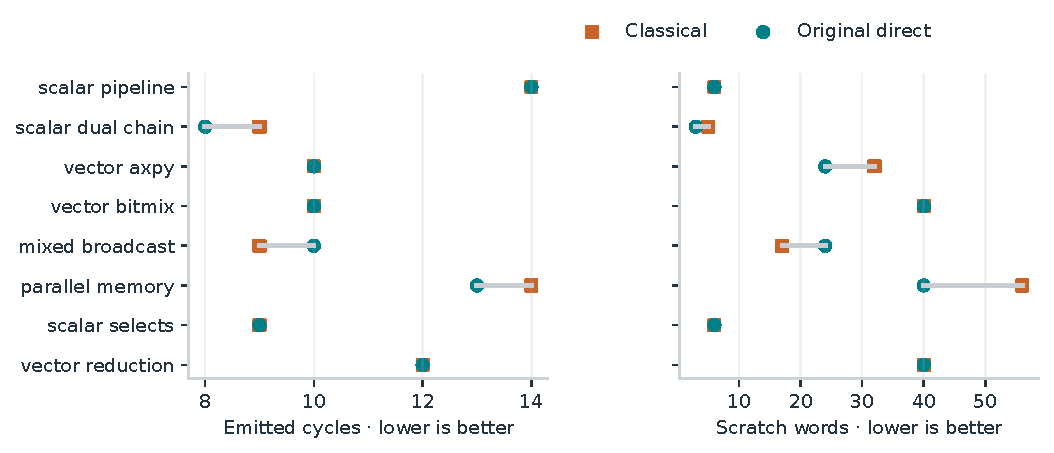
\includegraphics[width=.85\linewidth]{output_quality.pdf}
\caption{Phase 1, public programs: cycles and scratch words of the original direct
compiler against classical. Lower is better on both axes.}\label{fig:p1quality}
\end{figure}
\begin{figure}[htbp]\centering
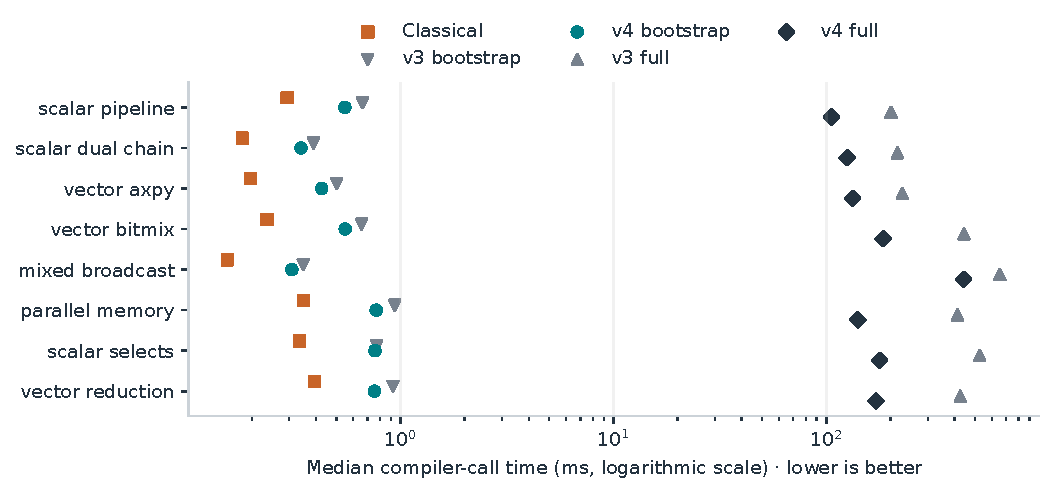
\includegraphics[width=.85\linewidth]{compile_times.pdf}
\caption{Phase 1: median compile-call times over \V{pOneReps} repetitions per public
program for classical and both versions of the direct compiler.}\label{fig:p1times}
\end{figure}
\begin{figure}[htbp]\centering
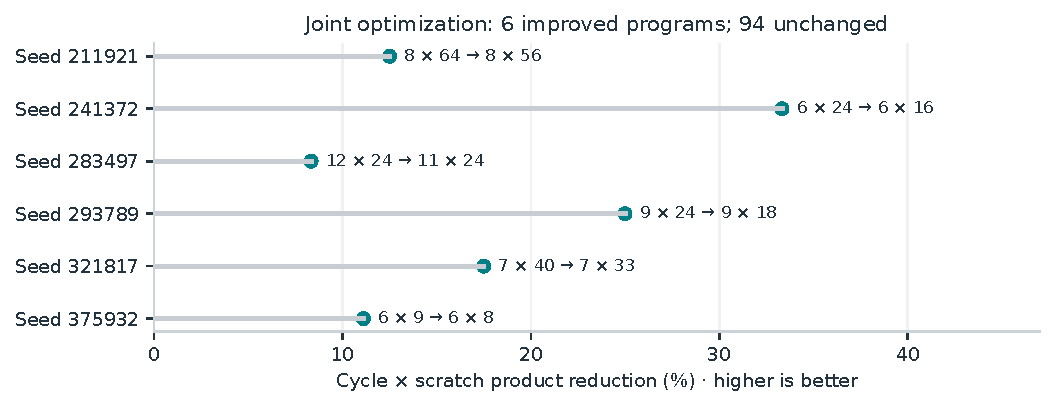
\includegraphics[width=.85\linewidth]{optimizer_ablation.pdf}
\caption{Phase 1: the generated programs improved by the bounded optimiser, with the
product before and after.}\label{fig:p1ablation}
\end{figure}
\begin{figure}[htbp]\centering
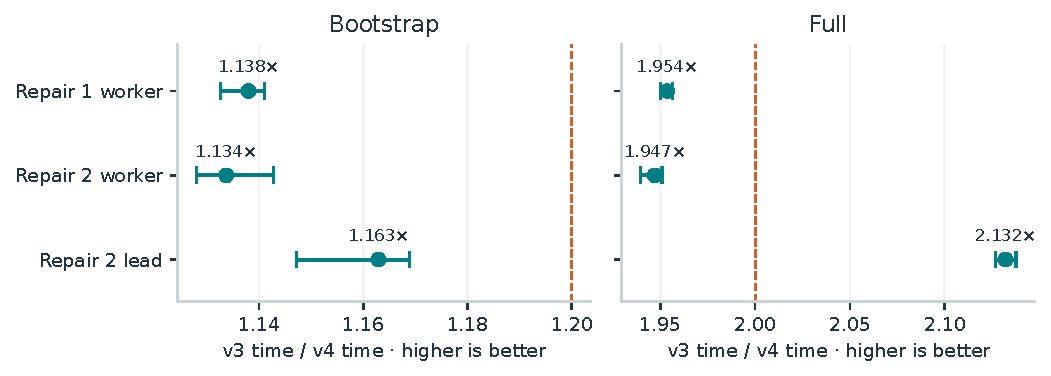
\includegraphics[width=.85\linewidth]{run_variability.pdf}
\caption{Phase 1: three runs of the same production code. Error bars are
within-run paired intervals and do not describe variation between runs.}
\label{fig:p1var}
\end{figure}
\FloatBarrier

\section{Structural-encoding feasibility}\label{sec:feasibility}

A separate, pre-declared campaign asked whether exact structural encodings of
whole-program choices could be sampled well enough to support later experiments.
Finite checks covered \V{feFixtures} fixtures, \V{feExhausted} exhausted code
universes and \V{feRoundTrips} round trips, with no failures. Two sampling streams per
public program retained \V{feAttempts} attempts in \V{feStreams} streams,
\V{feCompletions} completed draws and \V{feCaseChecks} case checks with
\V{feDiscrepancies} discrepancies; raw-bit sampling produced no completions. The gate
required \V{feMinimum} distinct completions per program, and \V{feBelow} programs fell
below it (Table~\ref{tab:feasibility}). The campaign is inconclusive: this sampler
did not pass its gate, which neither shows that structural encoding is impossible
nor establishes any compression or performance benefit. The later stages were
blocked and never measured.

\begin{table}[htbp]\centering\small
\begin{tabularx}{\linewidth}{Xrrrl}\toprule
Program & Raw-bit & Option-path & Distinct union & Gate\\\midrule
\tableinput{generated/phase2_coverage_rows.tex}
\bottomrule\end{tabularx}
\caption{Completed draws per stream and the distinct union across streams, by
public program.}\label{tab:feasibility}
\end{table}

\section{Review, errata and deviations}\label{sec:errata}

\paragraph{Self-review.} The acceptance of C1 was performed by the implementer
because the designated lead reviewer was unavailable; it is disclosed as a
self-review, and an independent re-review would supersede it.

\paragraph{Erratum E1.} The release handoff of the final round quotes a hash for C1
that matches no file or record in the repository; it was a transcription error.
The measured C1 is the file with SHA-256
\par\noindent{\small\texttt{\V{hCOne}}}\par\noindent which appears in both
freezes, the final source manifest and the export manifest.

\paragraph{Erratum E2.} The handoff states that the frozen development auditor is
an exact prefix of the current file. A later edit, made before the confirmation
freeze, changed two places inside that prefix. Running the development audit from
both files gives the same \V{tAuditD} checks in each case, with the frozen file's
own hash as the only finding, so the edit does not change the development audit.

\paragraph{Disclosed deviations.} The kernel draft preceded its specification; an
auditor was extended after the development freeze (E2); a false positive in the
cohort inventory was corrected before any outcome; one unused variable was left in
a frozen file to preserve its hash; development rows ran in a different order from
confirmation rows; two auditor tests were re-targeted, not weakened; a few smoke
runs were not charged to the ledger and are not evidence; and the cost-model
correction of Section~\ref{sec:third} is post hoc. None changes a gate.

\paragraph{Checks.} The confirmation audit passed \V{tAuditC} checks with no
findings and the repaired model audit \V{tAuditM}. The review ran \V{tPytest} tests of
the final round and \V{tInherited} inherited semantic tests, all passing, and checked
\V{tRawStdout} raw output streams against their rows.

\section{Artefacts and reproduction}\label{sec:artefacts}

The measured C1 source is \path{research/third_round_candidate.py}, with SHA-256
\par\noindent{\small\texttt{\V{hCOne}}}\par\noindent R0 is \path{research/efficiency_search.py}. The evidence of the
final round is under
\path{results/phase2_structural_encoding/third_round_20260925_resume/} and its review
under \path{results/phase2_structural_encoding/lead_resume_review_20260926/}. The
paper is rebuilt, without any new timing, by
\begin{verbatim}
venv/bin/python luminal-challenge/paper/build_paper.py
\end{verbatim}
which regenerates the figures, the tables and the value ledger, runs the worked
example through the real compilers, re-derives every ledger entry from its source
file, compiles both documents, and rejects unresolved references, overfull boxes
and any digit in the manuscript that does not come from the ledger. The challenge
asks that the exercise and its solution not be shared publicly, so these artefacts
are kept local.

\section{The claim ledger}\label{sec:ledger}

Every number in the main text and in this document is a macro whose value is
recorded below with the file it comes from and the field or derivation that
produces it. Pointer entries are re-read from disk and derived entries are
recomputed on every build; entries computed by the generators (the worked example
and the Phase 1 checks) are reproduced by rerunning them. Paths abbreviate
\path{results/phase2_structural_encoding/} as \path{p2/}.

{\scriptsize
\begin{longtable}{>{\raggedright\arraybackslash}p{32mm}>{\raggedright\arraybackslash}p{24mm}>{\raggedright\arraybackslash}p{53mm}>{\raggedright\arraybackslash}p{38mm}}
\toprule
Key & Value & Source & Field or derivation\\\midrule\endhead
\tableinput{generated/tab_ledger.tex}
\bottomrule
\end{longtable}}

\begin{thebibliography}{9}\raggedright\small
\bibitem{shaw1998} P. Shaw, \emph{Using Constraint Programming and Local Search
Methods to Solve Vehicle Routing Problems}, in \emph{Principles and Practice of
Constraint Programming -- CP98}, LNCS 1520 (Springer, 1998), pp. 417--431.
\url{https://doi.org/10.1007/3-540-49481-2_30}.
\bibitem{harvey1995} W. D. Harvey and M. L. Ginsberg, \emph{Limited Discrepancy
Search}, in \emph{Proceedings of IJCAI-95}, Vol. 1, pp. 607--613 (1995).
\bibitem{castaneda2019} R. Castañeda Lozano, M. Carlsson, G. Hjort Blindell and
C. Schulte, \emph{Combinatorial Register Allocation and Instruction Scheduling},
\emph{ACM TOPLAS} 41(3), Article 17 (2019). \url{https://doi.org/10.1145/3332373}.
\bibitem{ohrimenko2009} O. Ohrimenko, P. J. Stuckey and M. Codish,
\emph{Propagation via lazy clause generation}, \emph{Constraints} 14(3),
357--391 (2009). \url{https://doi.org/10.1007/s10601-008-9064-x}.
\bibitem{gasse2019} M. Gasse, D. Chételat, N. Ferroni, L. Charlin and A. Lodi,
\emph{Exact Combinatorial Optimization with Graph Convolutional Neural Networks},
NeurIPS 2019. \url{https://arxiv.org/abs/1906.01629}.
\bibitem{breiman1984} L. Breiman, J. H. Friedman, R. A. Olshen and C. J. Stone,
\emph{Classification and Regression Trees} (Wadsworth, 1984).
\end{thebibliography}
\end{document}
